\cleardoublepage
% \phantomsection
\addcontentsline{toc}{chapter}{Úvod}
\chapter*{Úvod}\label{chap:intro}

Dátové štruktúry a algoritmy tvoria základnú, prvotnú časť výučby 
informatiky. Vizualizácia algoritmov a dátových štruktúr je grafické 
znázornenie, ktoré abstrahuje od implementačných detailov a reprezentácie
v pamäti. Je teda vhodnou pomôckou pri výučbe i samoštúdiu. 

Ukážka nášho softvéru \emph{Gnarley Trees} je na obrázku~\ref{img:historia}.
Tento projekt začal ako bakalárska práca Jakuba Kováča \citep{kuko};
v tejto práci popisujeme nové dátové štruktúry, ktoré sme vizualizovali
a nové funkcie a vylepšenia, ktoré sme doplnili. Konkrétne ide o 
\emph{union-find problém}, \emph{písmenkový strom (trie)} a 
\emph{sufixový strom}. 

Softvér v súčasnosti vyvíja okrem Kuba Kováča aj Katka Kotrlová, ktorá 
vizualizovala rôzne typy háld a intervalové stromy, Táňa Tóthová, ktorá 
vizualizovala \emph{finger tree} a \emph{B$^+$-strom}.
Okrem vizualizácie softvér prerábame a neustále vylepšujeme.
Pavol Lukča ho doplnil o históriu krokov a operácií. Softvér je celý v 
slovenčine aj angličtine a je 
implementovaný v jazyku \Java. Dostupný je na stránke
{\url{http://people.ksp.sk/~kuko/gnarley-trees}} vo forme appletov
s jednotlivými dátovými štruktúrami, a tiež vo forme samostatného programu,
ktorý obsahuje všetky dátové štruktúry a je určený na používanie offline.

Našou snahou je vytvoriť kvalitný softvér nezávislý od operačného systému, 
ktorý bude vyhovovať ako pomôcka pri výučbe ako aj pri samoštúdiu a bude
voľne prístupný. 

%\bigskip
Predchádzajúci výskum v oblasti pedagogiky
zatiaľ nedokázal úplne preukázať pedagogickú efektívnosť
vizualizácií \citep{shaffer}, avšak viacero štúdií potvrdilo zvýšený záujem
a zapojenosť študentov \citep{naps02, hundhausen02}.

Rozmach vizualizácie algoritmov priniesla najmä \Java\ a jej fungovanie 
bez viazanosti na konkrétny operačný systém. Kvalita iných existujúcich 
vizualizácií sa líši a keďže ide o ľahko naprogramovateľné programy, je ich 
veľa a sú pomerne nekvalitné \citep{shaffer}. 
Zbieraním a analyzovaním kvality sa venuje skupina AlgoViz (\hbox{\url{http://algoviz.org/}}).

Zaujímavé je pozorovanie, že určovanie si vlastného tempa pri vizualizácií 
je veľká pomôcka. Naopak, ukazovanie pseudokódu alebo nemožnosť určenia si
vlastného tempa (napríklad animácia bez možnosti pozastavenia), takmer 
žiadne zlepšenie neprináša \citep{shaffer,saraiya}.

%\bigskip
% Zvyšok článku je organizovaný nasledovne: V sekcií 2 popisujeme implementované
% vylepšenia týkajúce sa vizualizácie, grafiky a ovládania, v sekciách 3 až 6
% nové dátové štruktúry, ktoré sme implementovali a vizualizovali: vyvážené
% stromy, haldy, union-find a písmenkové stromy.

Prácu sme rozdelili na popis jednotlivých dátových štruktúr, ktoré sme 
vizualizovali a popis samotného softvéru. V kapitolách~
\ref{chap:uf}, \ref{chap:trie} a \ref{chap:sx} je postupne popis 
\emph{union-find}, \emph{písmenkového stromu} a \emph{sufixového stromu}. 
V~kapitole~\ref{chap:popis} je popis softvéru a 
v~kapitole~\ref{chap:implementacia} je implementácia.
 
\begin{figure}
\centering
\greybox{%
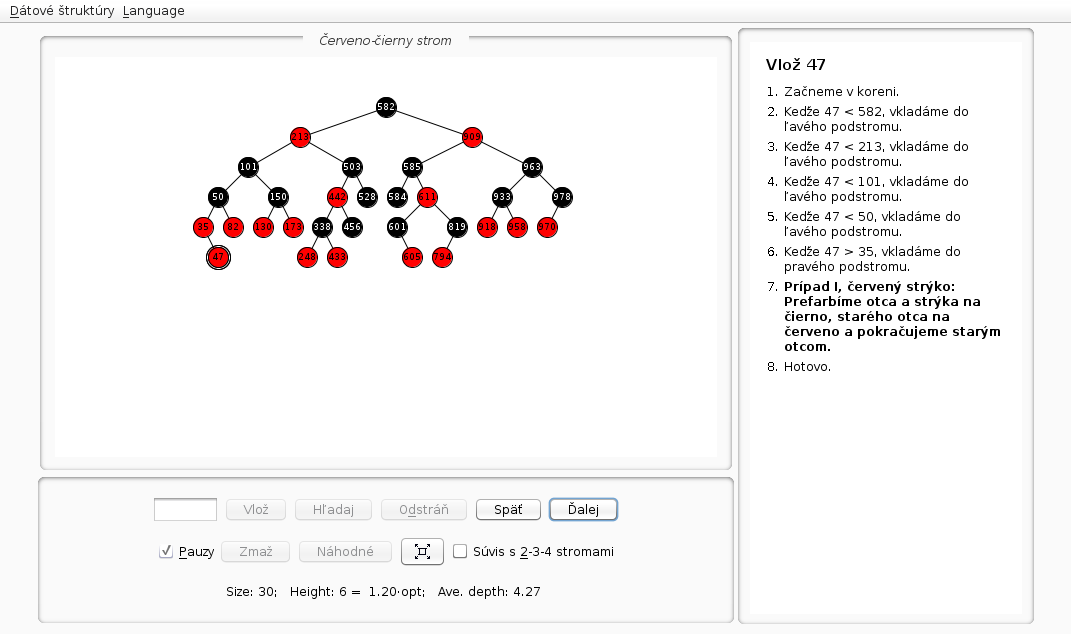
\includegraphics[width=\columnwidth]{obrazky/gt.png}%
}
\caption{\emph{Softvér Gnarley Trees.} V ovládacom paneli dole môže používateľ
zvoliť operáciu a vstupnú hodnotu a sledovať priebeh algoritmu (zobrazené je vkladanie
prvku 47). Používateľ postupuje vlastným tempom  pomocou tlačidiel \uv{Ďalej} alebo
\uv{Späť}. Vpravo je popis vykonávaných krokov; kliknutím na konkrétny krok v histórií
sa môže používateľ vrátiť.}
\label{img:historia} 
\end{figure}
